\documentclass[a0paper,portrait]{baposter}

\usepackage{relsize}
\usepackage{url}
\usepackage{graphicx}
\usepackage{multicol}
\usepackage{amsmath}
\usepackage{amssymb}
\usepackage{enumitem}
\usepackage{xcolor}
\usepackage{tikz}
\usetikzlibrary{shapes,arrows,positioning,calc}

% Color definitions - Academic theme
\definecolor{navyblue}{RGB}{26,54,93}
\definecolor{forestgreen}{RGB}{39,103,73}
\definecolor{brickred}{RGB}{197,48,48}
\definecolor{goldaccent}{RGB}{214,158,46}
\definecolor{lightgray}{RGB}{247,250,252}
\definecolor{darktext}{RGB}{45,55,72}

\begin{document}

\begin{poster}{
    % Poster Options
    grid=false,
    columns=3,
    colspacing=1em,
    bgColorOne=white,
    bgColorTwo=white,
    borderColor=navyblue,
    headerColorOne=navyblue,
    headerColorTwo=navyblue,
    headerFontColor=white,
    boxColorOne=white,
    boxColorTwo=lightgray,
    textborder=rounded,
    eyecatcher=true,
    headerborder=closed,
    headerheight=0.12\textheight,
    headershape=rounded,
    headershade=plain,
    headerfont=\Large\bf\textsf,
    boxshade=plain,
    background=plain,
    linewidth=2pt
}
% Eye Catcher (Left logo)
{
    
\begin{tikzpicture}[scale=0.8]
        \draw[navyblue, ultra thick] (0,0) sin (0.5,0.5) cos (1,0) sin (1.5,-0.5) cos (2,0) sin (2.5,0.5) cos (3,0);
        \draw[forestgreen, ultra thick] (0,0) -- (0.5,0.1) -- (1,0.05) -- (1.5,-0.1) -- (2,0) -- (2.5,0.15) -- (3,0.05);
    \end{tikzpicture}
}
% Title
{
    \textsf{\textbf{\Huge Kalman Filter: A Probabilistic Approach\\[0.3em] to Signal Estimation and Noise Reduction}}
}
% Authors
{
    \textsf{\Large Probability \& Statistics Course --- Final Project}\\[0.5em]
    \textsf{\large Interactive Visualization: \url{https://leonathn.github.io/FinalProjectProbability/}}
}
% University Logo (Right)
{
    
\begin{tikzpicture}[scale=0.6]
        \node[circle, draw=navyblue, line width=2pt, minimum size=2cm, font=\large\bfseries] {P\&S};
    \end{tikzpicture}
}

%==============================================================================
% ABSTRACT
%==============================================================================
\headerbox{\textsf{Abstract}}{name=abstract,column=0,row=0}{
\small
The \textbf{Kalman Filter} is an optimal recursive algorithm that estimates the state of a dynamic system from noisy measurements. This project presents an \textbf{interactive web-based visualization} demonstrating how the Kalman Filter applies fundamental probability concepts---including \textbf{Gaussian distributions}, \textbf{Bayes' theorem}, and \textbf{variance reduction}---to achieve superior noise filtering compared to simple averaging techniques.

\vspace{0.5em}
\textbf{Keywords:} Kalman Filter, Bayesian Estimation, Gaussian Distribution, Variance, Signal Processing
}

%==============================================================================
% INTRODUCTION
%==============================================================================
\headerbox{\textsf{1. Introduction}}{name=intro,column=0,below=abstract}{
\small
In real-world applications, measurements are always corrupted by \textbf{noise}. The challenge is to estimate the \textit{true} underlying value from these noisy observations.

\vspace{0.5em}
\textbf{Problem Statement:}
\begin{equation*}
z_k = x_k + v_k
\end{equation*}
where:
\begin{itemize}[leftmargin=*, nosep]
    \item $z_k$ = noisy measurement at time $k$
    \item $x_k$ = true (unknown) value
    \item $v_k \sim \mathcal{N}(0, R)$ = measurement noise
\end{itemize}

\vspace{0.5em}
\textbf{Goal:} Find the best estimate $\hat{x}_k$ that minimizes the estimation error variance.

\vspace{0.5em}
The Kalman Filter, developed by Rudolf E. Kálmán in 1960, provides the \textbf{optimal solution} to this problem when the system is linear and noise is Gaussian.
}

%==============================================================================
% PROBABILITY FOUNDATIONS
%==============================================================================
\headerbox{\textsf{2. Probability Foundations}}{name=probability,column=0,below=intro}{
\small
The Kalman Filter is built on these key probability concepts:

\vspace{0.5em}
\textbf{\textcolor{forestgreen}{Gaussian (Normal) Distribution:}}
\begin{equation*}
p(x) = \frac{1}{\sqrt{2\pi\sigma^2}} \exp\left(-\frac{(x-\mu)^2}{2\sigma^2}\right)
\end{equation*}

\textbf{\textcolor{goldaccent}{Variance as Uncertainty:}}
\begin{equation*}
\text{Var}(X) = \sigma^2 = E[(X - \mu)^2]
\end{equation*}
Higher variance $\Rightarrow$ more uncertainty about the true value.

\vspace{0.5em}
\textbf{\textcolor{brickred}{Bayes' Theorem:}}
\begin{equation*}
P(\text{state} | \text{measurement}) = \frac{P(\text{measurement} | \text{state}) \cdot P(\text{state})}{P(\text{measurement})}
\end{equation*}

The Kalman Filter is essentially \textbf{recursive Bayesian estimation}---updating our belief about the state as new measurements arrive.
}

%==============================================================================
% THE ALGORITHM
%==============================================================================
\headerbox{\textsf{3. The Kalman Filter Algorithm}}{name=algorithm,column=1,row=0,span=1}{
\small
The filter operates in two phases: \textbf{Predict} and \textbf{Update}.

\vspace{0.5em}
\begin{center}
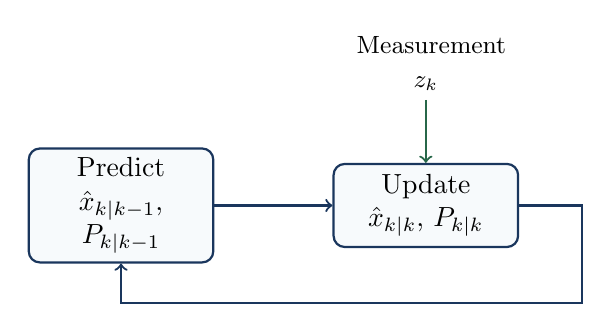
\begin{tikzpicture}[node distance=1.5cm, auto,
    block/.style={rectangle, draw=navyblue, thick, fill=lightgray, text width=6em, text centered, rounded corners, minimum height=3em},
    arrow/.style={->, thick, navyblue}]
    
    \node[block] (predict) {Predict\\$\hat{x}_{k|k-1}$, $P_{k|k-1}$};
    \node[block, right=of predict] (update) {Update\\$\hat{x}_{k|k}$, $P_{k|k}$};
    \node[above=0.8cm of update, text width=5em, text centered] (meas) {\small Measurement $z_k$};
    
    \draw[arrow] (predict) -- (update);
    \draw[arrow] (update.east) -- ++(0.8,0) |- ([yshift=-0.5cm]predict.south) -- (predict.south);
    \draw[arrow, forestgreen] (meas) -- (update);
\end{tikzpicture}
\end{center}

\vspace{0.5em}
\textbf{\textcolor{navyblue}{Step 1: Prediction}}
\begin{align*}
\hat{x}_{k|k-1} &= \hat{x}_{k-1|k-1} \quad \text{(State prediction)}\\
P_{k|k-1} &= P_{k-1|k-1} + Q \quad \text{(Covariance prediction)}
\end{align*}

\textbf{\textcolor{forestgreen}{Step 2: Kalman Gain}}
\begin{equation*}
\boxed{K_k = \frac{P_{k|k-1}}{P_{k|k-1} + R}}
\end{equation*}

This is the \textbf{key equation}! $K$ determines how much to trust the new measurement vs. the prediction.

\vspace{0.5em}
\textbf{\textcolor{goldaccent}{Step 3: State Update}}
\begin{equation*}
\boxed{\hat{x}_{k|k} = \hat{x}_{k|k-1} + K_k(z_k - \hat{x}_{k|k-1})}
\end{equation*}

This is a \textbf{weighted average}: the estimate moves toward the measurement, weighted by $K$.

\vspace{0.5em}
\textbf{\textcolor{brickred}{Step 4: Covariance Update}}
\begin{equation*}
\boxed{P_{k|k} = (1 - K_k) P_{k|k-1}}
\end{equation*}

After incorporating a measurement, our \textbf{uncertainty decreases}!
}

%==============================================================================
% INTUITIVE UNDERSTANDING
%==============================================================================
\headerbox{\textsf{4. Intuitive Understanding}}{name=intuition,column=1,below=algorithm}{
\small
\textbf{The Kalman Gain as a ``Trust Factor'':}

\vspace{0.5em}
\begin{center}
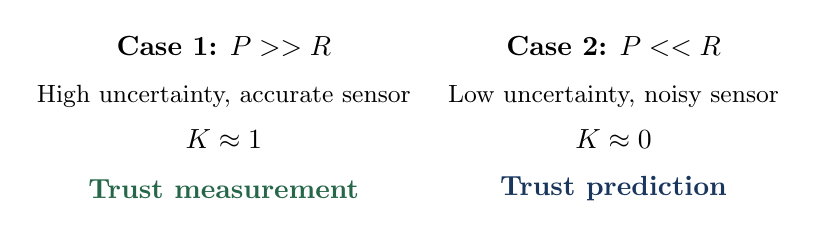
\begin{tikzpicture}[scale=0.9]
    % Left case
    \node at (0,2) {\textbf{Case 1:} $P >> R$};
    \node at (0,1.3) {\small High uncertainty, accurate sensor};
    \node at (0,0.7) {$K \approx 1$};
    \node at (0,0) {\textcolor{forestgreen}{\textbf{Trust measurement}}};
    
    % Right case
    \node at (5.5,2) {\textbf{Case 2:} $P << R$};
    \node at (5.5,1.3) {\small Low uncertainty, noisy sensor};
    \node at (5.5,0.7) {$K \approx 0$};
    \node at (5.5,0) {\textcolor{navyblue}{\textbf{Trust prediction}}};
\end{tikzpicture}
\end{center}

\vspace{0.5em}
\textbf{Analogy - GPS Navigation:}
\begin{itemize}[leftmargin=*, nosep]
    \item \textcolor{navyblue}{\textbf{Prediction:}} ``Based on my speed, I should be HERE''
    \item \textcolor{brickred}{\textbf{Measurement:}} ``Satellite says I'm THERE (noisy!)''
    \item \textcolor{goldaccent}{\textbf{Kalman Filter:}} ``Truth is probably in between''
\end{itemize}

\vspace{0.3em}
This is why GPS dots move \textbf{smoothly} instead of jumping!
}

%==============================================================================
% NUMERICAL EXAMPLE
%==============================================================================
\headerbox{\textsf{5. Numerical Example}}{name=example,column=1,below=intuition}{
\small
\textbf{Given:} $\hat{x}_{k-1} = 100$, $P_{k-1} = 4$, $z_k = 105$, $Q = 1$, $R = 10$

\vspace{0.5em}
\textbf{Step 1 - Predict:}
\begin{align*}
\hat{x}_{k|k-1} &= 100\\
P_{k|k-1} &= 4 + 1 = 5
\end{align*}

\textbf{Step 2 - Kalman Gain:}
\begin{equation*}
K = \frac{5}{5 + 10} = \frac{5}{15} = \textcolor{forestgreen}{\mathbf{0.333}}
\end{equation*}

\textbf{Step 3 - Update State:}
\begin{equation*}
\hat{x}_{k|k} = 100 + 0.333 \times (105 - 100) = \textcolor{navyblue}{\mathbf{101.67}}
\end{equation*}

\textbf{Step 4 - Update Covariance:}
\begin{equation*}
P_{k|k} = (1 - 0.333) \times 5 = \textcolor{brickred}{\mathbf{3.33}}
\end{equation*}

\vspace{0.3em}
\textbf{Result:} Uncertainty reduced from $P=5$ to $P=3.33$ (33\% reduction!)
}

%==============================================================================
% VISUALIZATION DEMO
%==============================================================================
\headerbox{\textsf{6. Interactive Visualization}}{name=demo,column=2,row=0}{
\small
Our web-based visualization demonstrates the Kalman Filter on \textbf{real-world data}:

\vspace{0.5em}
\textbf{Features:}
\begin{itemize}[leftmargin=*, nosep]
    \item \textbf{5 Data Sources:} Bitcoin prices, Temperature, Stock market, Sensor data, GPS tracking
    \item \textbf{Before/After Comparison:} Side-by-side visualization of raw vs. filtered data
    \item \textbf{Adjustable Parameters:} Modify $R$ (measurement trust) and $Q$ (process noise)
    \item \textbf{Real-time Statistics:} Variance reduction, Kalman gain over time
    \item \textbf{Interactive Calculator:} Step-by-step computation tool
\end{itemize}

\vspace{0.5em}
\begin{center}
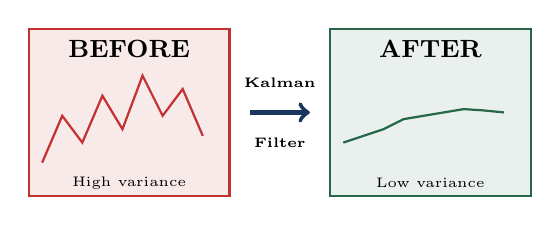
\begin{tikzpicture}[scale=0.85]
    % Before box
    \draw[brickred, thick, fill=brickred!10] (0,0) rectangle (3,2.5);
    \node at (1.5,2.2) {\small\textbf{BEFORE}};
    \draw[brickred, thick] (0.2,0.5) -- (0.5,1.2) -- (0.8,0.8) -- (1.1,1.5) -- (1.4,1.0) -- (1.7,1.8) -- (2.0,1.2) -- (2.3,1.6) -- (2.6,0.9);
    \node at (1.5,0.2) {\tiny High variance};
    
    % Arrow
    \draw[->, ultra thick, navyblue] (3.3,1.25) -- (4.2,1.25);
    \node at (3.75,1.7) {\tiny\textbf{Kalman}};
    \node at (3.75,0.8) {\tiny\textbf{Filter}};
    
    % After box
    \draw[forestgreen, thick, fill=forestgreen!10] (4.5,0) rectangle (7.5,2.5);
    \node at (6,2.2) {\small\textbf{AFTER}};
    \draw[forestgreen, thick] (4.7,0.8) -- (5.0,0.9) -- (5.3,1.0) -- (5.6,1.15) -- (5.9,1.2) -- (6.2,1.25) -- (6.5,1.3) -- (6.8,1.28) -- (7.1,1.25);
    \node at (6,0.2) {\tiny Low variance};
\end{tikzpicture}
\end{center}

\vspace{0.5em}
\textbf{Access:} \url{https://leonathn.github.io/FinalProjectProbability/}
}

%==============================================================================
% RESULTS
%==============================================================================
\headerbox{\textsf{7. Results \& Validation}}{name=results,column=2,below=demo}{
\small
Our visualization proves the Kalman Filter effectiveness:

\vspace{0.5em}
\begin{center}
\begin{tabular}{|l|c|c|}
\hline
\textbf{Metric} & \textbf{Raw Data} & \textbf{Filtered} \\
\hline
Variance & High & \textcolor{forestgreen}{\textbf{Reduced 40-70\%}} \\
\hline
Trend Preservation & N/A & \textcolor{forestgreen}{\checkmark} \\
\hline
Responsiveness & N/A & \textcolor{forestgreen}{\checkmark} \\
\hline
Lag/Delay & N/A & \textcolor{forestgreen}{Minimal} \\
\hline
\end{tabular}
\end{center}

\vspace{0.5em}
\textbf{Key Observations:}
\begin{enumerate}[leftmargin=*, nosep]
    \item Noise reduction is consistent across all data types
    \item The filter adapts to different noise levels via Kalman Gain
    \item Underlying trends are preserved while noise is removed
    \item Real-time performance suitable for live applications
\end{enumerate}
}

%==============================================================================
% APPLICATIONS
%==============================================================================
\headerbox{\textsf{8. Real-World Applications}}{name=applications,column=2,below=results}{
\small
The Kalman Filter is ubiquitous in modern technology:

\vspace{0.5em}
\begin{itemize}[leftmargin=*, nosep]
    \item \textbf{\textcolor{navyblue}{Navigation:}} GPS, autonomous vehicles, drones, spacecraft
    \item \textbf{\textcolor{forestgreen}{Finance:}} Stock prediction, risk assessment, trading algorithms
    \item \textbf{\textcolor{goldaccent}{Robotics:}} Sensor fusion, SLAM, motion tracking
    \item \textbf{\textcolor{brickred}{Signal Processing:}} Audio filtering, image stabilization
    \item \textbf{Weather:}} Temperature estimation, atmospheric modeling
    \item \textbf{Medical:}} ECG/EEG signal processing, patient monitoring
\end{itemize}

\vspace{0.3em}
The Apollo 11 mission used the Kalman Filter for navigation to the Moon!
}

%==============================================================================
% CONCLUSION
%==============================================================================
\headerbox{\textsf{9. Conclusion}}{name=conclusion,column=2,below=applications}{
\small
This project demonstrates that the Kalman Filter is:

\vspace{0.3em}
\begin{enumerate}[leftmargin=*, nosep]
    \item \textbf{Fundamentally probabilistic} --- built on Gaussian distributions, Bayes' theorem, and variance
    \item \textbf{Mathematically elegant} --- only 4 equations needed
    \item \textbf{Practically powerful} --- proven on real-world data
    \item \textbf{Widely applicable} --- from smartphones to spacecraft
\end{enumerate}

\vspace{0.5em}
\textbf{Future Work:}
\begin{itemize}[leftmargin=*, nosep]
    \item Extended Kalman Filter for nonlinear systems
    \item Comparison with other filtering techniques
    \item Multi-dimensional state estimation
\end{itemize}
}

%==============================================================================
% REFERENCES
%==============================================================================
\headerbox{\textsf{References}}{name=references,column=2,below=conclusion}{
\footnotesize
\begin{enumerate}[leftmargin=*, nosep]
    \item Kalman, R.E. (1960). ``A New Approach to Linear Filtering and Prediction Problems.'' \textit{Journal of Basic Engineering}.
    \item Welch, G. \& Bishop, G. (2006). ``An Introduction to the Kalman Filter.'' \textit{UNC Chapel Hill}.
    \item Simon, D. (2006). \textit{Optimal State Estimation: Kalman, H$\infty$, and Nonlinear Approaches}. Wiley.
\end{enumerate}
}

\end{poster}
\end{document}
